\documentclass[10pt,a4]{article}

\title{KPM Semester project - 10}
\author{Tomáš Hadwiger, Tomáš Calábek}
\date{}

\usepackage{listings}
\usepackage{pdfpages}
\usepackage{hyperref}

\begin{document}
    \maketitle
    \section{Our task \& objectives}
    The objective of this project was to create a comprehensive network scenario using the 5G-LENA module of the NS3 simulator, configure the parameters of the network, and analyze the network performance.
    %%% maybe write out the objectives?
    \section{Network Scenario}
    Our network scenario (see \hyperref[fig:network]{Figure 1}) was made of 5 UEs and 2 gNodeBs. Two of the UEs were streaming video from a remote host over the Internet, while the other three UEs were browsing the web.
    Our network was further comprised of 2 gNodeBs, with maximum of three UE connections per single gNodeB.
    \begin{figure}[ht!]
        \centering
        \caption{A diagram of the network scenario.}
        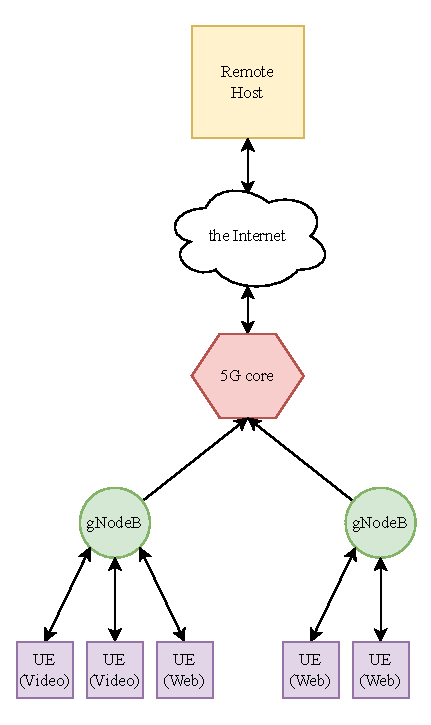
\includegraphics[height=0.6\textwidth]{../kpm-plots/network.pdf}
        \label{fig:network}
    \end{figure}
    \section{Configuration}
    \subsection*{Parameters}
    A short list of the most releveant parameters for our simulation, as well as their default values, can be seen in \hyperref[lst:params]{Listing 1}. These values can be modified with command line arguments when running the script using NS3 syntax.
    \begin{lstlisting}[language=C++,caption=Relevant default parameters.,label=lst:params][ht!]
    uint32_t udpPacketSizeBrowsing = 25; // bytes
    uint32_t udpPacketSizeVideo = 50;    // bytes
    uint32_t lambdaBrowsing = 10000;     // packets per sec
    uint32_t lambdaVideo = 10000;        // packets per sec
    double totalTxPower = 35.0;          // dBm
    \end{lstlisting}
    Our script utilizes a sub-6GHz frequency band, as per the assignment. The sub-6GHz band is said to typically ranges from 410 MHz to 7125 MHz. This frequency band offers wide coverage and better penetration through obstacles when compared to the mmWave band and, while it delivers slower transfer speeds compared to the mmWave, its speed is still a significant improvement over 4G. We use central frequency of 2.8 GHz for video streaming and 2.82 GHz for web browsing.

    Further, we also take advantage of two numerologies, one for each type of communication (e.g. video streaming and web browsing). For video streaming we utilize numerology 4, while for web browsing the numerology 2 is used. This corresponds to subcarrier spacing of 240 kHz and 60 kHz respectively.

    Lastly, we set up apropriate IPv4 addresses and ranges for all the devices in the network. Our PGW is connected to the remote host using a Point-to-Point link and is assigned the address 8.0.0.0 with the subnet mask of 255.0.0.0; the UEs are assigned address from a 7.0.0.0 IP range.
    \subsection*{Traffic generation}
    According to our assignment, the traffic on the network should be comprised of web browsing and video streaming. To this end, we create two dedicated bearers with the appropriate traffic flow templates (e.g. \texttt{GBR\_CONV\_VIDEO} for video streaming and \texttt{NGBR\_LOW\_LAT\_EMBB} for web browsing) assigned to each. The traffic flow templates ensure appropriate traffic flow and QoS (Quality of Service) are used to each type of communication.

    The communication itself is facilliates by an UDP server installed onto the remote host and a UDP client installed onto the UEs.
    \begin{lstlisting}[language=C++,caption=Traffic bearer definition.,label=lst:tfts][ht!]
    NrEpsBearer bearerBrowsing(NrEpsBearer::NGBR_LOW_LAT_EMBB);
    NrEpsBearer bearerVideo(NrEpsBearer::GBR_CONV_VIDEO);
    \end{lstlisting}
    \section{Flow analysis results}
    To quantify our results, we use the FlowMonitor tool, which is an integral part of the NS3 simulator. We capture key metrics, like data speed, packet loss and throughput, into logs which we then use to analyze the impact of various parameters onto the network performance.

    The FlowMonitor tool collects vast amounts of data for each simulation run, so for clarity we only include some of the most interesting results of our many simulation runs.

    tohle jeste musim dodelat, ale to bude nudny a zabere to vterinu
    \section{REM analysis}
    The REM (Radio Environment Map) is a tool in NS3 which generates maps of the radio environment, that help with visualizing signal propagation, intereference patterns and coverage with the network.

    While many different modes, and thus different data points, of the REM are possible, we only focus on two:
    \begin{itemize}
        \item \textbf{Beam Shape}: this mode allows us to visualize the shape of the beam in terms of SNR/SINR map;
        \item \textbf{Coverage Area}: this mode produces the best-case SNR (visualizes best possible beams) and worst-case SINR scenario (assuming all devices are pointing towards the REM point) for each REM point;
        \item \textbf{UE Coverage}: this mode works in the uplink direction (e.g. UE is the transmitter) and assumes the beams of the other gNodeBs are pointed towards the receiving gNodeB.
    \end{itemize}

    The results of our simulation are shown on \hyperref[fig:dl]{Figure 2} and \hyperref[fig:ul]{Figure 3}.

    Unforunately, when creating the REM map for UL UE Coverage scenario, the simulation persistently crashed with error show in \hyperref[lst:error]{Listing 3}. -- \textbf{TOHLE MUSI CHECKNOUT CALDA NA VMce}

    \begin{lstlisting}[language=C++,caption=Error produced by NS3 when generating UL UE Coverage REM,label=lst:error]
    NS_ASSERT failed, cond="m_spectrumModel == x.m_spectrumModel",
    +0.100000000s -1
    file=~/Vut/kpm/ns-3-dev/src/spectrum/model/spectrum-value.cc,
    line=107
    NS_FATAL, terminating
    \end{lstlisting}

    \begin{figure}[ht!]
    \caption{REM map results in downlink direction.}
    \label{fig:dl}
    \resizebox{\textwidth}{!}{\begin{tabular}{r|cccc}
    & IPSD & SNR & SINR & SIR \\
    \hline
    \textbf{Beam Shape} &
    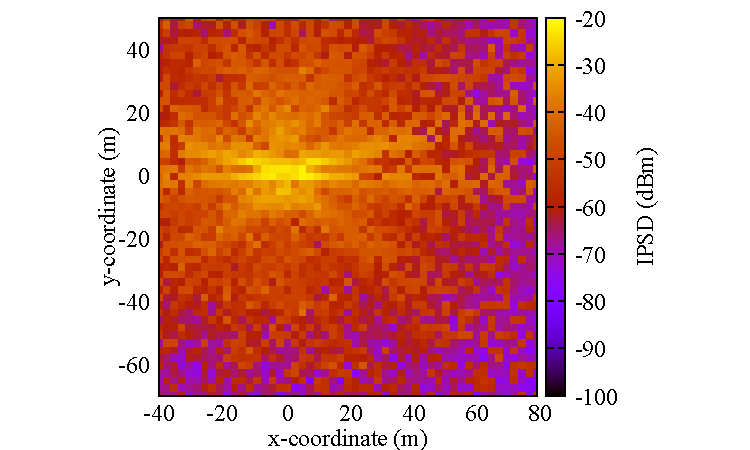
\includegraphics[width=0.25\linewidth]{../kpm-plots/nr-rem-DL_BEAM_SHAPE-ipsd.pdf} &
    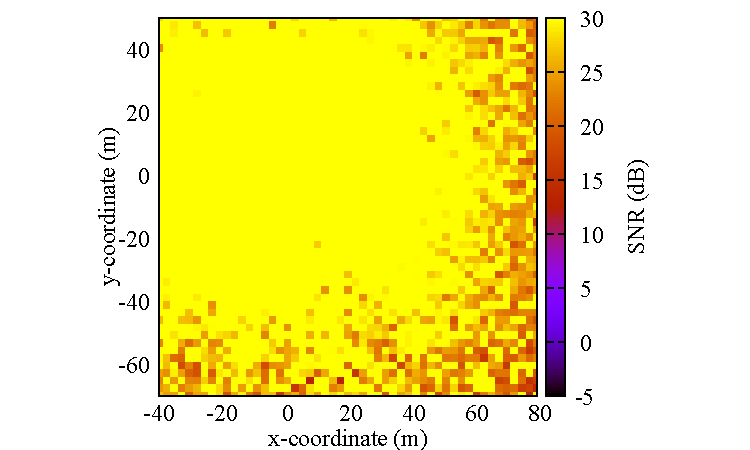
\includegraphics[width=0.25\linewidth]{../kpm-plots/nr-rem-DL_BEAM_SHAPE-snr.pdf} &
    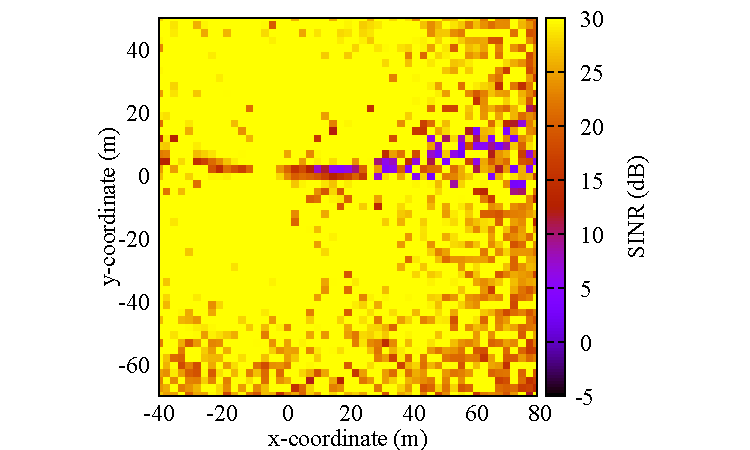
\includegraphics[width=0.25\linewidth]{../kpm-plots/nr-rem-DL_BEAM_SHAPE-sinr.pdf} &
    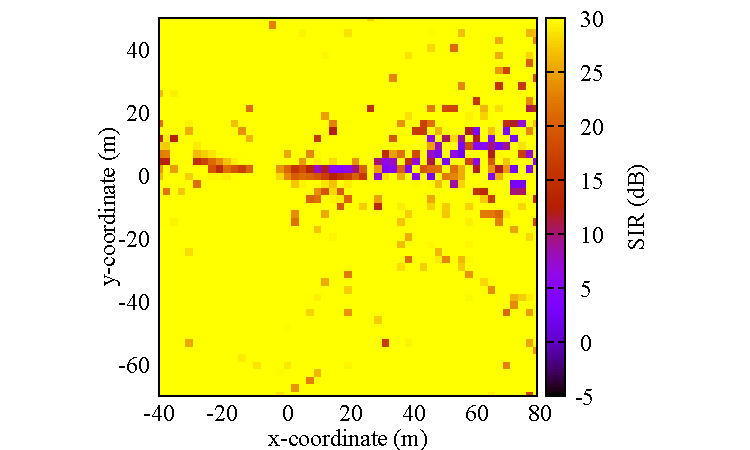
\includegraphics[width=0.25\linewidth]{../kpm-plots/nr-rem-DL_BEAM_SHAPE-sir.pdf} \\
    \hline
    \textbf{Coverage Area} &
    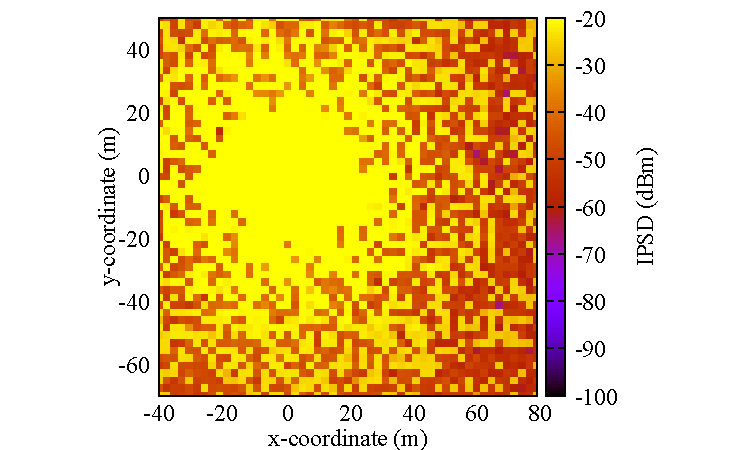
\includegraphics[width=0.25\linewidth]{../kpm-plots/nr-rem-DL_COVERAGE_AREA-ipsd.pdf} &
    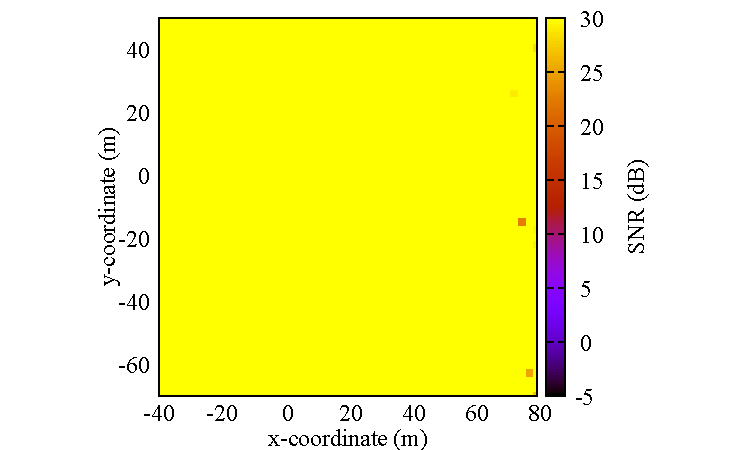
\includegraphics[width=0.25\linewidth]{../kpm-plots/nr-rem-DL_COVERAGE_AREA-snr.pdf} &
    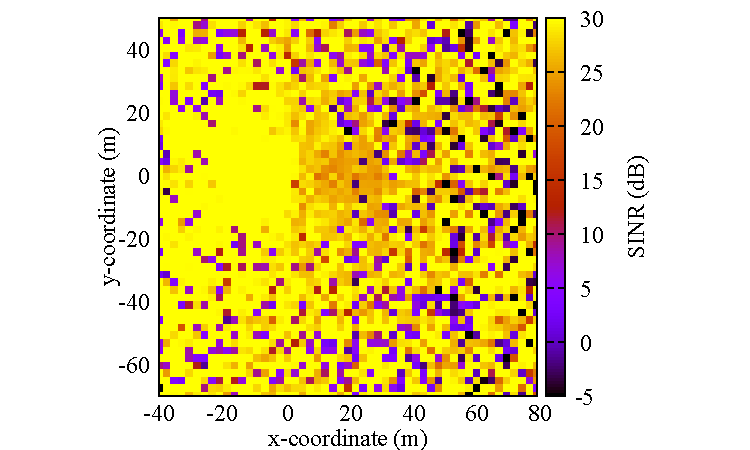
\includegraphics[width=0.25\linewidth]{../kpm-plots/nr-rem-DL_COVERAGE_AREA-sinr.pdf} &
    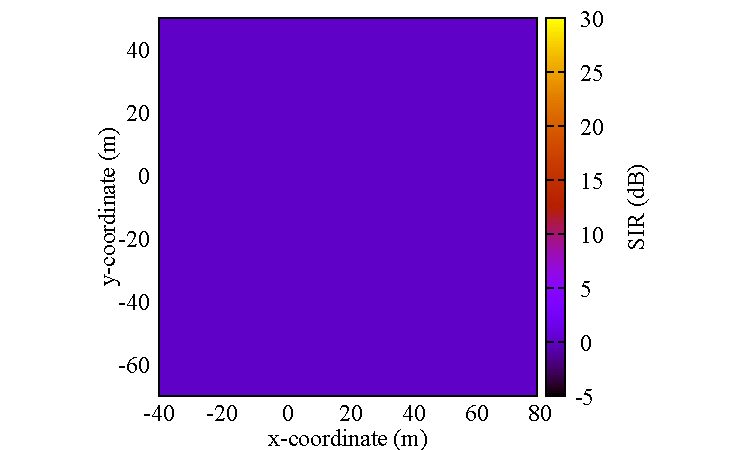
\includegraphics[width=0.25\linewidth]{../kpm-plots/nr-rem-DL_COVERAGE_AREA-sir.pdf} \\
    \hline
    \textbf{UE Coverage} &
    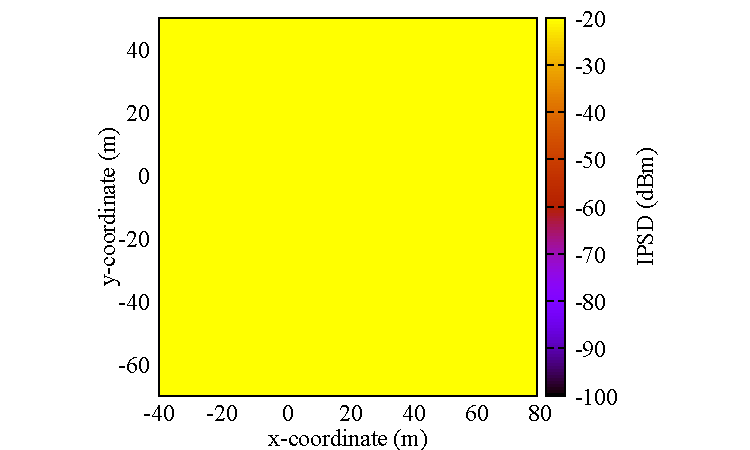
\includegraphics[width=0.25\linewidth]{../kpm-plots/nr-rem-DL_UE_COVERAGE-ipsd.pdf} &
    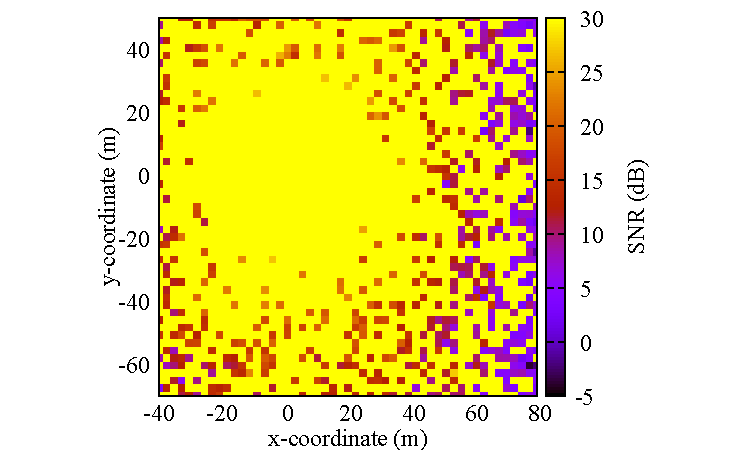
\includegraphics[width=0.25\linewidth]{../kpm-plots/nr-rem-DL_UE_COVERAGE-snr.pdf} &
    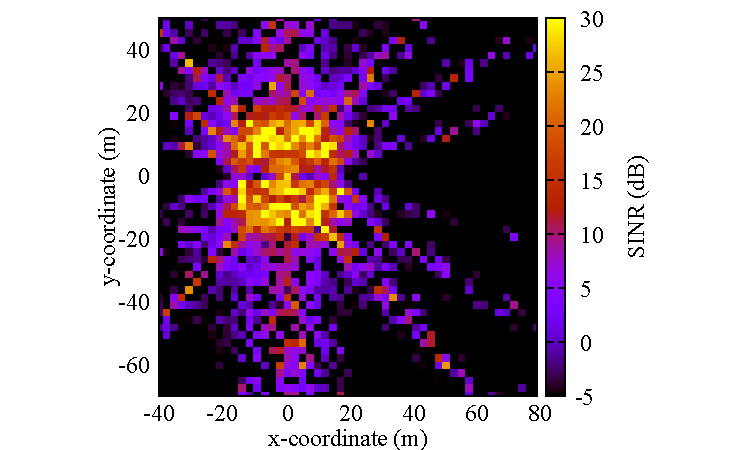
\includegraphics[width=0.25\linewidth]{../kpm-plots/nr-rem-DL_UE_COVERAGE-sinr.pdf} &
    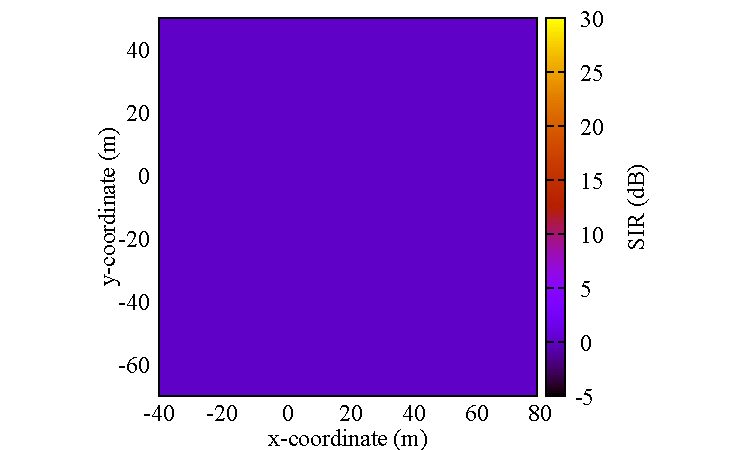
\includegraphics[width=0.25\linewidth]{../kpm-plots/nr-rem-DL_UE_COVERAGE-sir.pdf} \\
    \end{tabular}}
    \end{figure}



    \begin{figure}[ht!]
    \caption{REM map results in uplinkdirection.}
    \label{fig:ul}
    \resizebox{\textwidth}{!}{\begin{tabular}{r|cccc}
    & IPSD & SNR & SINR & SIR \\
    \hline
    \textbf{Beam Shape} &
    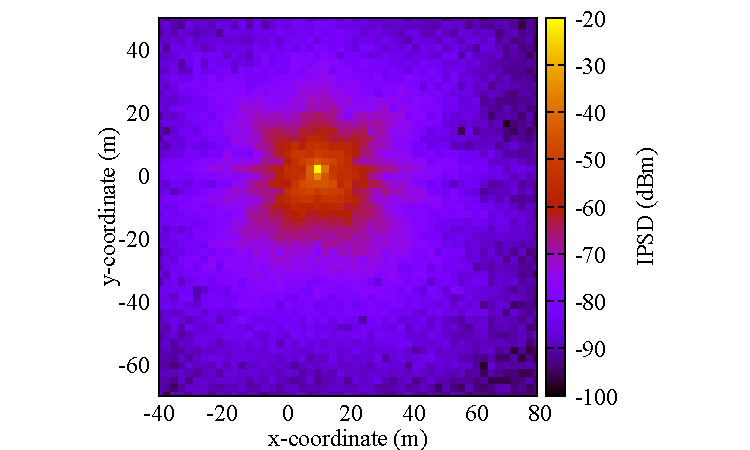
\includegraphics[width=0.25\linewidth]{../kpm-plots/nr-rem-UL_BEAM_SHAPE-ipsd.pdf} &
    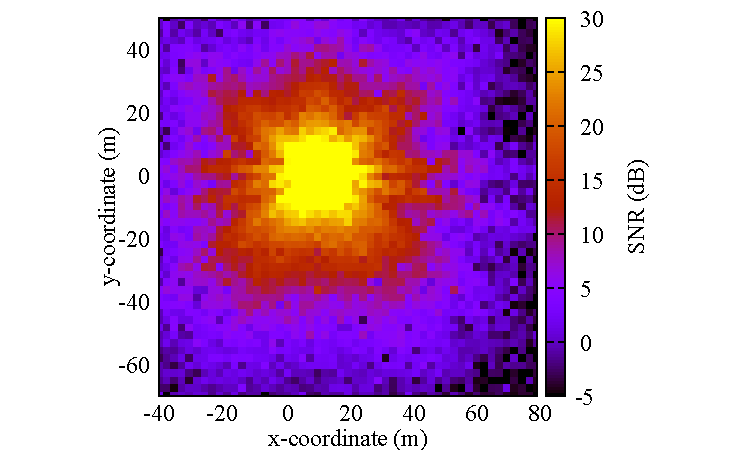
\includegraphics[width=0.25\linewidth]{../kpm-plots/nr-rem-UL_BEAM_SHAPE-snr.pdf} &
    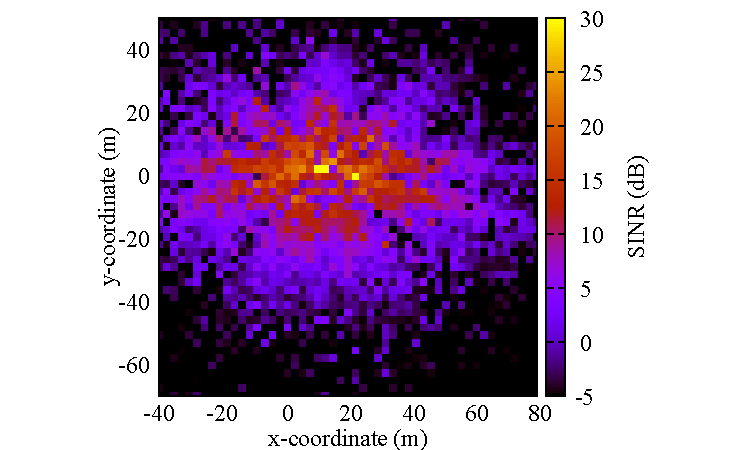
\includegraphics[width=0.25\linewidth]{../kpm-plots/nr-rem-UL_BEAM_SHAPE-sinr.pdf} &
    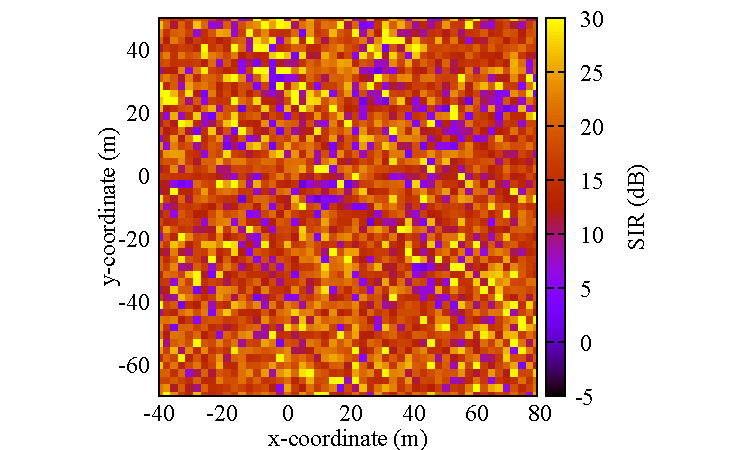
\includegraphics[width=0.25\linewidth]{../kpm-plots/nr-rem-UL_BEAM_SHAPE-sir.pdf} \\
    \hline
    \textbf{Coverage Area} &
    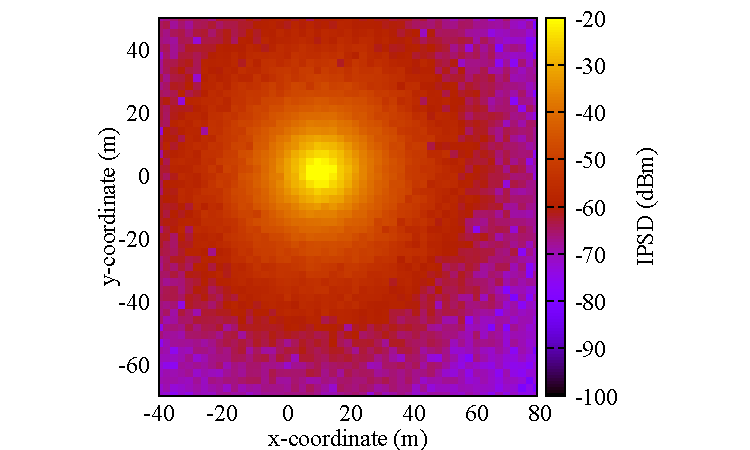
\includegraphics[width=0.25\linewidth]{../kpm-plots/nr-rem-UL_COVERAGE_AREA-ipsd.pdf} &
    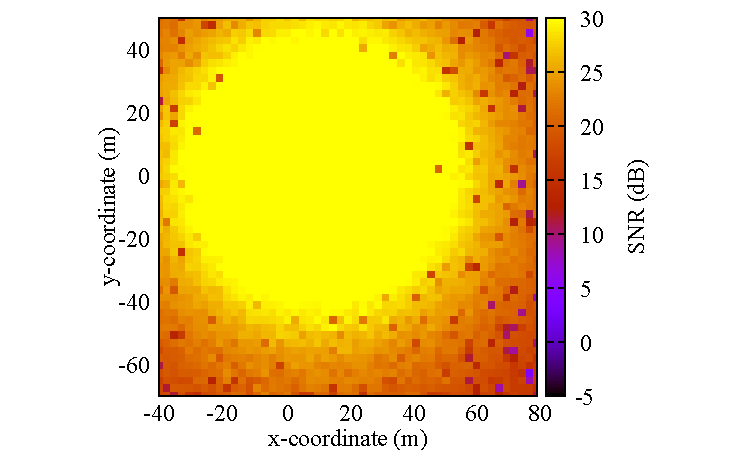
\includegraphics[width=0.25\linewidth]{../kpm-plots/nr-rem-UL_COVERAGE_AREA-snr.pdf} &
    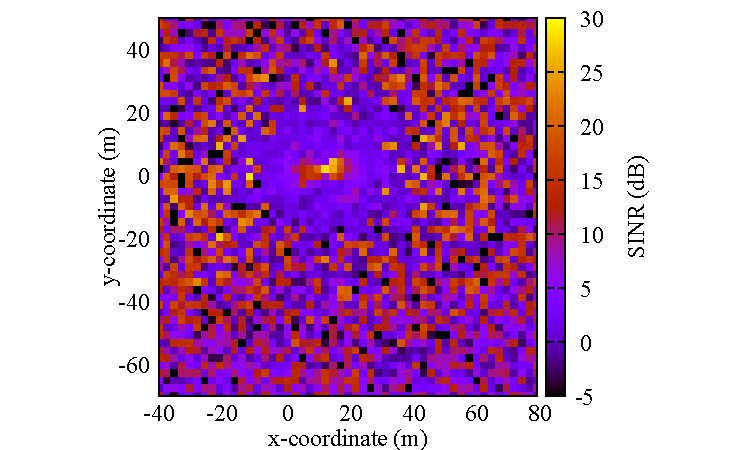
\includegraphics[width=0.25\linewidth]{../kpm-plots/nr-rem-UL_COVERAGE_AREA-sinr.pdf} &
    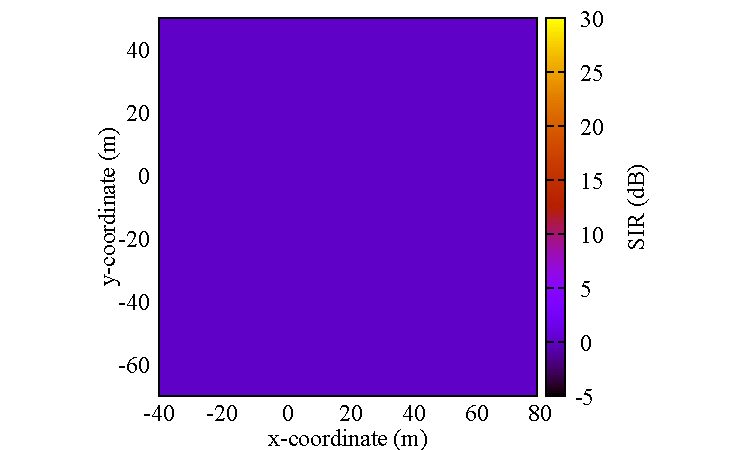
\includegraphics[width=0.25\linewidth]{../kpm-plots/nr-rem-UL_COVERAGE_AREA-sir.pdf} \\
    \hline
    \textbf{UE Coverage} &
    - &
    - &
    - &
    - \\
    \end{tabular}}
    \end{figure}
    \section{Challenges in working with NS3}
    Overall, working with the NS3 simulator and the 5G-LENA plugin wasn't extremely difficult, but it did provide a challenge, especially due to some lacking documentation on the parts of the 5G-LENA plugin.
    \section{Final insights}
    While our setup in NS3 does much to simulate the real world, it still cannot account for all the complex real variations of wireless transmission, especially when it comes to the complexity of the network (our scenario only includes 5 UEs and two gNodeBs, while in reality, you could have hundreds of UE devices connected to a single gNodeB). Further, our scenario assumes the UEs are in a fixed position over the duration of the communication which isn't always true in real world scenarios. Our script also uses idealized models for propagation and intereference, which do not fully model real factors like weather patterns, obstacles and device variability in terms of antennas.

    Both of us were somewhat familiar with the C++ language and NS3-specific syntax thanks to the laboratory excercises and this project only helped to further our understanding of both.
\end{document}
